\documentclass[footheight=20pt, footsepline, headheight=20pt, headsepline]{scrartcl}
%
\usepackage[utf8]{inputenc} % below are various important packages
\usepackage{lmodern}
\usepackage[T1]{fontenc}
\usepackage[english]{babel}
\usepackage{textcomp} 
\usepackage{amsmath}
\usepackage{mathrsfs}
\usepackage{listings}
\usepackage{latexsym}
\usepackage{amssymb}	
\usepackage{amsfonts}
\usepackage{float}
\usepackage{theorem}
\usepackage{graphicx}
\usepackage{placeins}
\usepackage{scrlayer-scrpage}
\usepackage{xcolor}
\usepackage{setspace}
\usepackage{framed}
\usepackage{hyperref} 
\usepackage{pgf,tikz,pgfplots} % possibility to insert geogebra graphs
\usepackage{mathrsfs}
\pgfplotsset{compat=1.15}\usetikzlibrary{arrows} % part of geogebra package
\usepackage{qrcode} % insert qr codes
\usepackage{multicol}
\usepackage{multirow}
\usepackage{xurl}
\usepackage{tabularx}
\usepackage{enumitem}
\usepackage{float}
\usepackage{colortbl,rotating,booktabs} % required packages for Excel2Latex


% Add to length for wider margins
\addtolength{\textwidth}{3cm} % right to margin
\addtolength{\hoffset}{-1.6cm} % left to margin
\addtolength{\voffset}{-2cm} % to top
\addtolength{\textheight}{6.5cm} % to bottom

% Headers-Footers
\definecolor{gro}{gray}{0.6} % define color
\setkomafont{pagehead}{\normalfont\sffamily} % define header
\setkomafont{pagefoot}{\normalfont\sffamily} % define footer
\addtokomafont{headsepline}{\color{gro}} % define header horizontal line



\renewcommand{\familydefault}{\sfdefault} % font
\linespread{1.2} % increase line spacing
%---------------------------------------------------------------------------
\begin{document} % every document starts with \begin{document}
%\doublespacing
\title{LAB REPORT (Lab-4) \\[1cm] \large{\textbf{CSE 3113: Microprocessor and Assembly Language Lab}}\\[1cm]} 
\author{Jahir Sadik Monon \\ Roll - 32}
\date{\vspace{10cm}  Submitted to, \\[0.1cm] Dr. Upama Kabir \\[0.5cm] Department of Computer Science and Engineering \\[0.5cm] University Of Dhaka}
\maketitle
\newpage
\tableofcontents 
%---------------------------------------------------------------------------
\newpage
\section*{Task 1}
\addcontentsline{toc}{section}{Task 1}
\textbf{Problem Statement:} Explain two directives: Data and Align with proper example.
\addcontentsline{toc}{subsection}{Problem Statement}
\subsection*{Explanation of DATA directive}
\addcontentsline{toc}{subsection}{Explanation of DATA directive}
\textbf{DATA}\\
The \verb|DATA| directive informs the assembler that a label is a data-in-code label. This means that the label is the address of data within a code segment.\\
The syntax of \verb|DATA| is\\
\textup{label} \verb|DATA|\\
where \textup{label} is the label of the data definition. The \verb|DATA| directive must be on the same line as \textup{label}.
\begin{lstlisting}
                        AREA            task1, CODE
                        ; code
                        ; code
                        MOV             pc, lr
                              DATA
                        DCB             1, 2, 3
\end{lstlisting}
\subsection*{Explanation of ALIGN directive}
\addcontentsline{toc}{subsection}{Explanation of ALIGN directive}
\textbf{ALIGN}\\
The \verb|ALIGN| directive is used to ensure the data and code is aligned to appropriate boundaries. This directive aligns the current location to a specified boundary by padding with zeros or \verb|NOP| instructions.\\
The syntax of \verb|ALIGN| is\\
\verb|ALIGN {expr{,offset{,pad{,padsize}}}}|\\
where \\
\verb|expr| is a numeric expression evaluating to any power of 2 from 2\textsuperscript{0} to 2\textsuperscript{31}.\\
\verb|offset| can be any numeric expression.\\
\verb|pad| can be any numeric expression.\\
\verb|padsize| can be 1, 2 or 4.
\begin{lstlisting}
        AREA    task1, CODE
        DCB     1      ; This example places the two bytes in the 
        ALIGN   4,3    ; first and fourth bytes of the same word.
        DCB     1      ; The second DCB is offset by 3 bytes from the first DCB.                        
\end{lstlisting}
%--------------------------------------------------------------------------------

\newpage
\FloatBarrier
\section*{Task 2}
\addcontentsline{toc}{section}{Task 2}
\textbf{Problem Statement:} Write an assembly program to display the status of each bit of the register PSR.
\addcontentsline{toc}{subsection}{Problem Statement}
\subsection*{Explanation of Code}
\addcontentsline{toc}{subsection}{Explanation of Code}
I have used the \verb|ADDS| instruction to set the flag values. Then I've used the \verb|MRS| instruction to move the status register values from iPSR, aPSR and ePSR to register.
\subsection*{Description of Instructions}
\addcontentsline{toc}{subsection}{Description of Instructions}
\textbf{MOV}\\The \verb|MOV| instruction copies the value of \verb|Operand2| into \verb|Rd|.\\
\verb|MOV{S}{cond} Rd, Operand2|\\
\verb|MOV{cond} Rd, #imm16|\\
\textbf{ADDS}\\
The \verb|ADD| instruction adds the values in Rn and Operand2 or imm12. \verb|S| is an optional suffix. If \verb|S| is specified, the condition flags are updated on the result of the operation.\\
\verb|ADD{S}{cond} {Rd}, Rn, Operand2|\\
\textbf{MUL}\\
Move the contents of a PSR to a general-purpose register.\\
\verb |MRS{cond} Rd, psr|\\




\FloatBarrier
\subsection*{Screenshot of the state \& status registers of the system after the code has been loaded}
\addcontentsline{toc}{subsection}{Screenshot of the state \& status registers of the system after the code has been loaded}
\begin{figure}[ht]
    \centering
    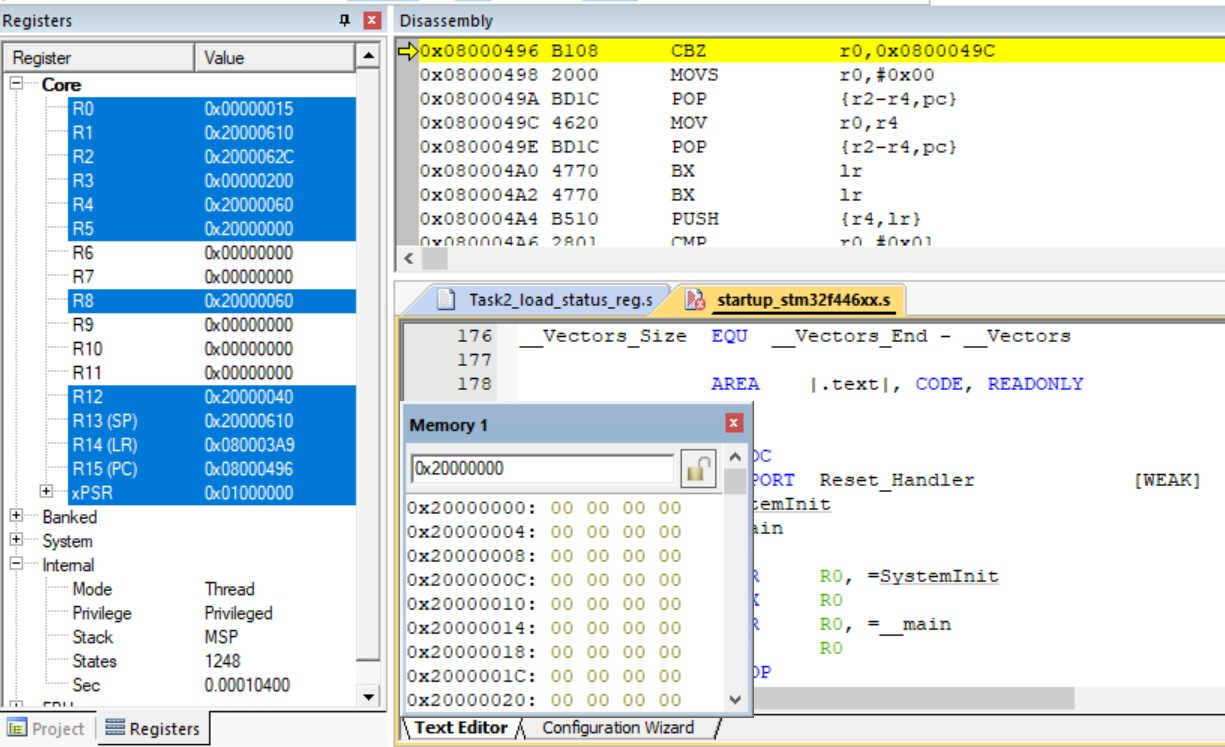
\includegraphics[scale=.7]{images/Task2_Before1.jpg}
    \caption{After loading the code on the system}
    \label{fig:before_task_3a}
\end{figure}
\FloatBarrier
\begin{figure}[ht]
    \centering
    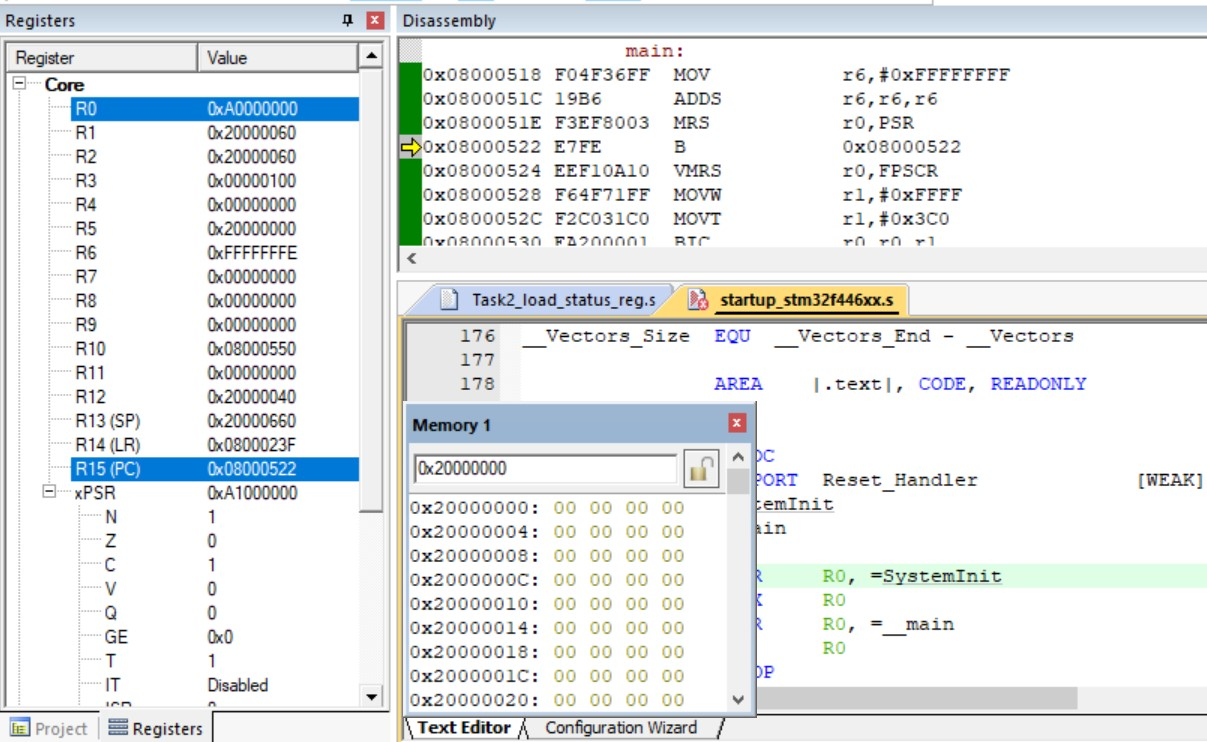
\includegraphics[scale=.7]{images/Task2_Before2.jpg}
    \caption{After loading the code on the system}
    \label{fig:before_task_3a}
\end{figure}
\FloatBarrier

\subsection*{Screenshot of the state of the system after the code has been executed}
\addcontentsline{toc}{subsection}{Screenshot of the state \& status registers of the system after the code has been executed}
\begin{figure}[h!]
    \centering
    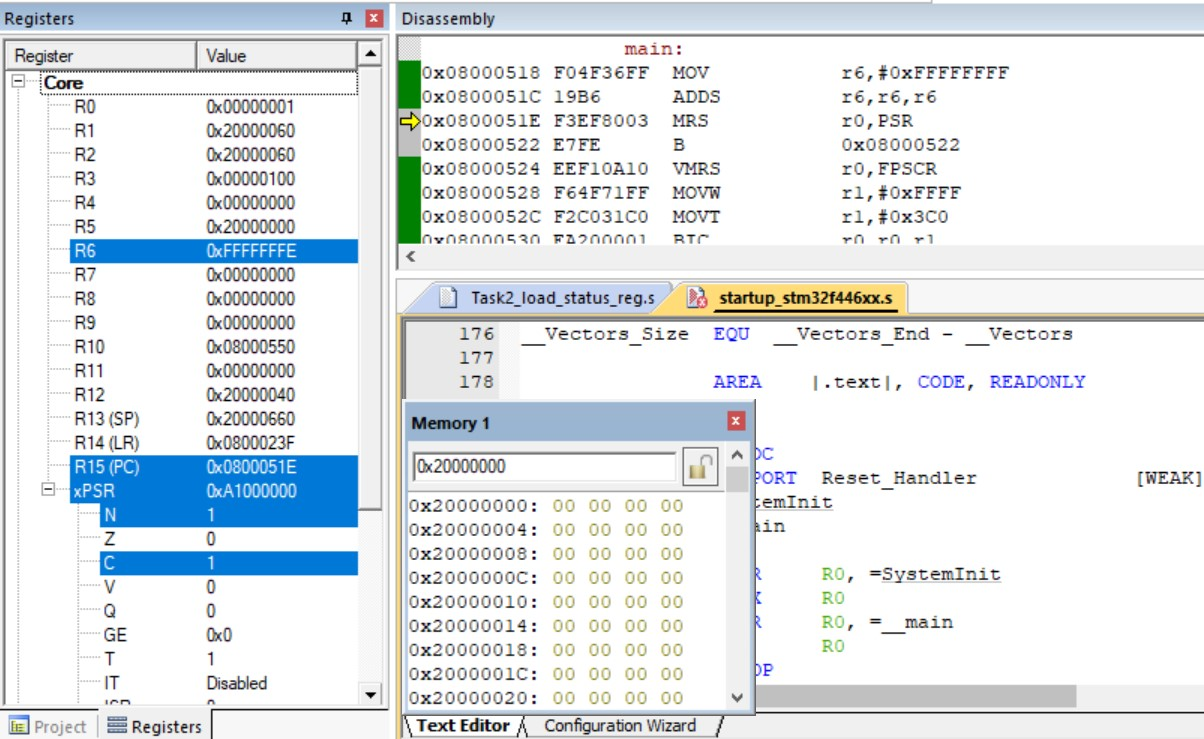
\includegraphics[scale=.7]{images/Task2_After1.jpg}
    \caption{After executing the code on the system}
    \label{fig:after_task_3a}
\end{figure}
\FloatBarrier
As we can see from the screenshot that the prior values of status registers is loaded into the \verb|$r0| register using MRS instruction.


%----------------------------------------------------------------------------------
\newpage
\FloatBarrier
\section*{Task iii(a)}
\addcontentsline{toc}{section}{Task iii(a)}
\textbf{Problem Statement:} Write an assembly program where the data is declared in Data region and the result will be in Data region.
\[ S = \sum_{i=1}^{10} i^{2} \]
\addcontentsline{toc}{subsection}{Problem Statement}
\subsection*{Explanation of Code}
\addcontentsline{toc}{subsection}{Explanation of Code}
The values of the sum (initially zero) and the loop endpoint are loaded into registers. We iterate over the values of \verb|i| and increment it in each iteration. If the value of \verb|i| exceeds the endpoint, we terminate the loop and store the resultant sum in memory. Otherwise, we add the squared value of \verb|i| to the sum and continue iterating.
\subsection*{Description of Instructions}
\addcontentsline{toc}{subsection}{Description of Instructions}
\textbf{MOV}\\The \verb|MOV| instruction copies the value of \verb|Operand2| into \verb|Rd|.\\
\verb|MOV{S}{cond} Rd, Operand2|\\
\verb|MOV{cond} Rd, #imm16|\\
\textbf{ADD}\\
The \verb|ADD| instruction adds the values in Rn and Operand2 or imm12. \verb|S| is an optional suffix. If \verb|S| is specified, the condition flags are updated on the result of the operation.\\
\verb|ADD{S}{cond} {Rd}, Rn, Operand2|\\
\textbf{MUL}\\
The \verb|MUL| istruction multiplies the values from Rn and Rm, and places the least significant 32 bits of he result in Rd.\\
\verb |MUL{S}{cond} {Rd}, Rn, Rm|\\
\textbf{LDR}\\
The \verb|LDR| pseudo-instruction loads a register with either a 32-bit constant value or an address.\\
\verb|LDR{type}{cond} Rt, [Rn {, #offset}]| \\
\textbf{STR}\\
The \verb|STR| pseudo-instruction loads a register with values from either a 32-bit constant or an address.\\
\verb|STR{type}{cond} Rt, [Rn {, #offset}]|\\  
\textbf{CMP}\\
The \verb|CMP| instruction subtracts the value of Operand2 from the value in Rn. This is the same as a \verb|SUBS| instruction, except that the result is discarded.\\
\verb|CMP{cond} Rn, Operand2|\\
\textbf{BGE}\\
The \verb|BGE| instruction performs branching to a label when the flag values for greater than are set to true.
\verb|BGE label|\\
\textbf{DCD}\\
The \verb|DCD| directive allocates one or more words of memory, aligned on four-byte boundaries, and defines the initial runtime contents of the memory.\\
\verb|{label} DCD{U} expr{,expr}|\\



\FloatBarrier
\subsection*{Screenshot of the state \& status registers of the system after the code has been loaded}
\addcontentsline{toc}{subsection}{Screenshot of the state \& status registers of the system after the code has been loaded}
\begin{figure}[ht]
    \centering
    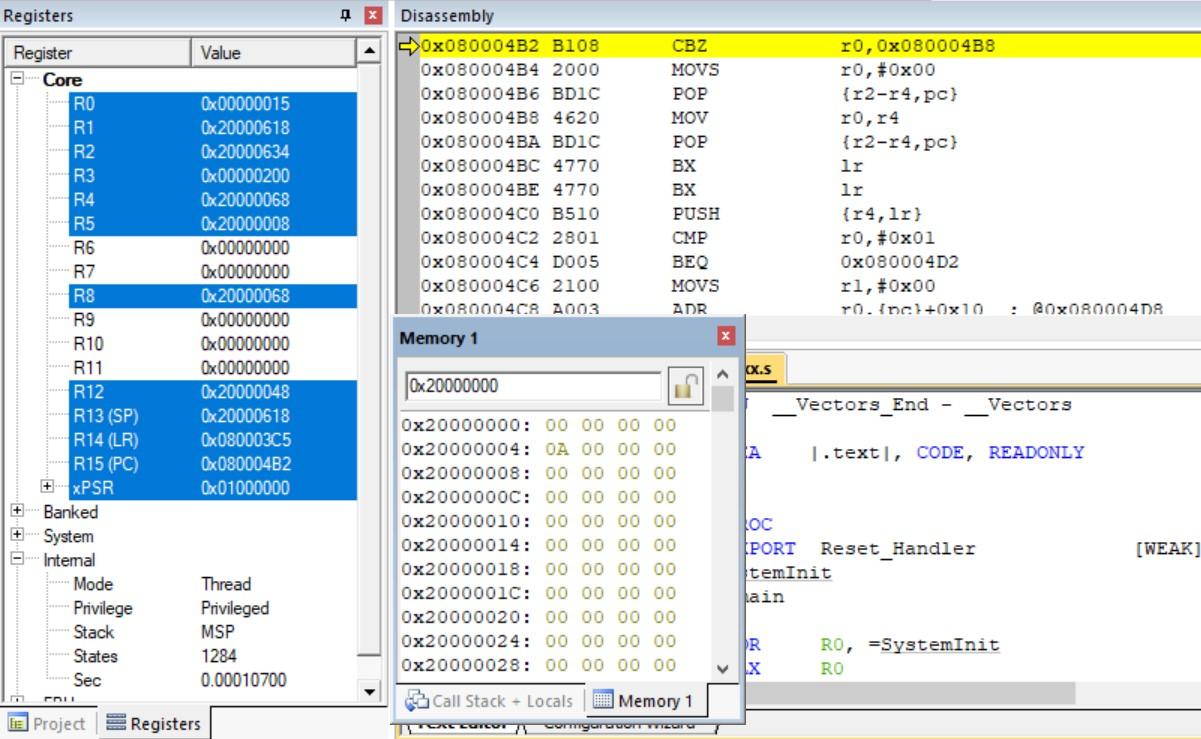
\includegraphics[scale=.7]{images/Task3a_Before1.jpg}
    \caption{After loading the code on the system}
    \label{fig:before_task_3a}
\end{figure}
\FloatBarrier
Here we can see that the registers are loaded with random values as the program is only loaded to the system and not executed yet. But the memory holds the value for S = 10 or 0x0A.
\subsection*{Screenshot of the state of the system after the code has been executed}
\addcontentsline{toc}{subsection}{Screenshot of the state \& status registers of the system after the code has been executed}
\begin{figure}[h!]
    \centering
    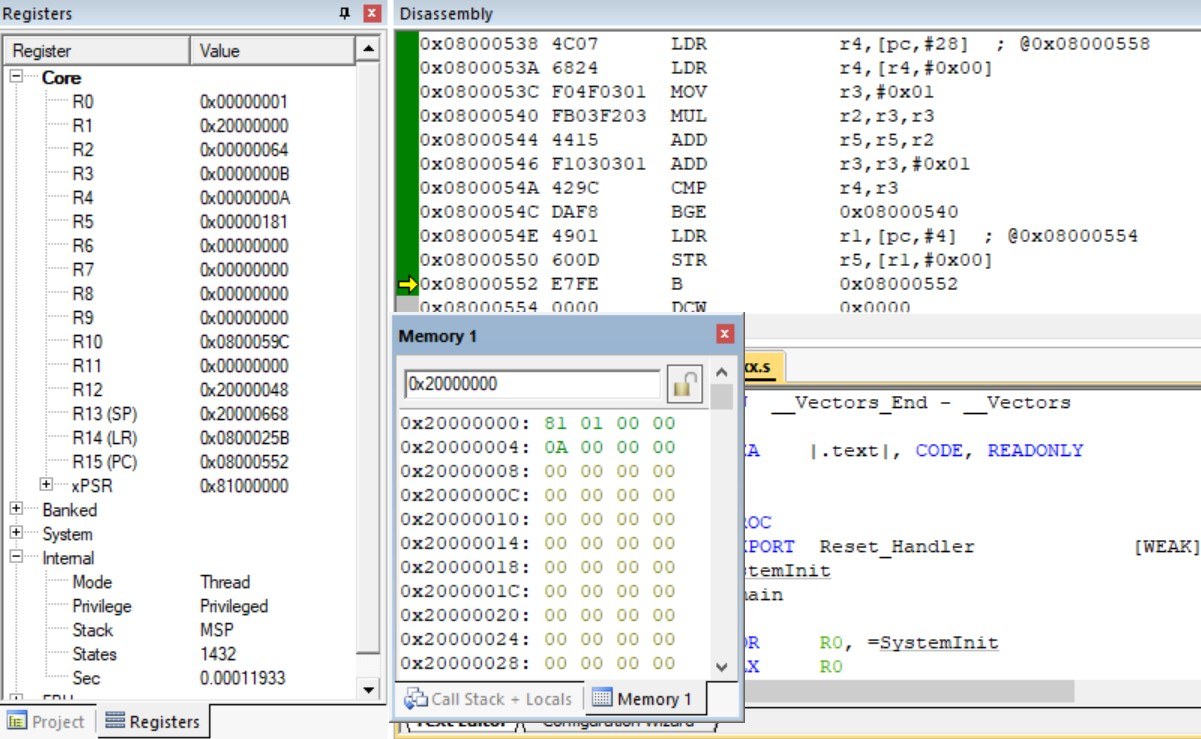
\includegraphics[scale=.7]{images/Task3a_After1.jpg}
    \caption{After executing the code on the system}
    \label{fig:after_task_3a}
\end{figure}
\FloatBarrier
As we can see, the register \$r5 as well as the memory holds the value 0x181, which should be the result of the operation. The memory value is in little-endian, thus the reverse view where it's showing 8101.








%------------------------------------------------------------------------------------
\FloatBarrier
\addcontentsline{toc}{section}{Task iii(b)}
\section*{Task iii(b)}
\addcontentsline{toc}{subsection}{Problem Statement}
\textbf{Problem Statement:} Write an assembly program where the data is declared in Data region and the result will be in Data region. The Pythagoras Theorem,\\
\[ a^2 =  b^2 + c^2\]
\subsection*{Explanation of Code}
\addcontentsline{toc}{subsection}{Explanation of Code}
The values of two sides (base and height) of a right-angled triangle are loaded into registers from memory. The sum of their squares is calculated and stored into another register, which matches the squared value of the hypotenuse of the triangle, thus verifying the Pythagoras theorem.\\
\subsection*{Description of Instructions}
\addcontentsline{toc}{subsection}{Description of Instructions}
\textbf{MOV}\\The \verb|MOV| instruction copies the value of \verb|Operand2| into \verb|Rd|.\\
\verb|MOV{S}{cond} Rd, Operand2|\\
\verb|MOV{cond} Rd, #imm16|\\
\textbf{ADD}\\
The \verb|ADD| instruction adds the values in Rn and Operand2 or imm12. \verb|S| is an optional suffix. If \verb|S| is specified, the condition flags are updated on the result of the operation.\\
\verb|ADD{S}{cond} {Rd}, Rn, Operand2|\\
\textbf{MUL}\\
The \verb|MUL| istruction multiplies the values from Rn and Rm, and places the least significant 32 bits of he result in Rd.\\
\verb |MUL{S}{cond} {Rd}, Rn, Rm|\\
\textbf{LDR}\\
The \verb|LDR| pseudo-instruction loads a register with either a 32-bit constant value or an address.\\
\verb|LDR{type}{cond} Rt, [Rn {, #offset}]| \\
\textbf{STR}\\
The \verb|STR| pseudo-instruction loads a register with values from either a 32-bit constant or an address.\\
\verb|STR{type}{cond} Rt, [Rn {, #offset}]|\\  
\textbf{DCDU}\\
The \verb|DCD| directive allocates one or more words of memory, aligned on four-byte boundaries, and defines the initial runtime contents of the memory.\verb|DCDU| is the same, except that the memory alignment is arbitrary.\\
\verb|{label} DCDU expr{,expr}|\\


\FloatBarrier
\subsection*{Screenshot of the state \& status registers of the system after the code has been loaded}
\addcontentsline{toc}{subsection}{Screenshot of the state \& status registers of the system after the code has been loaded}
\begin{figure}[ht]
    \centering
    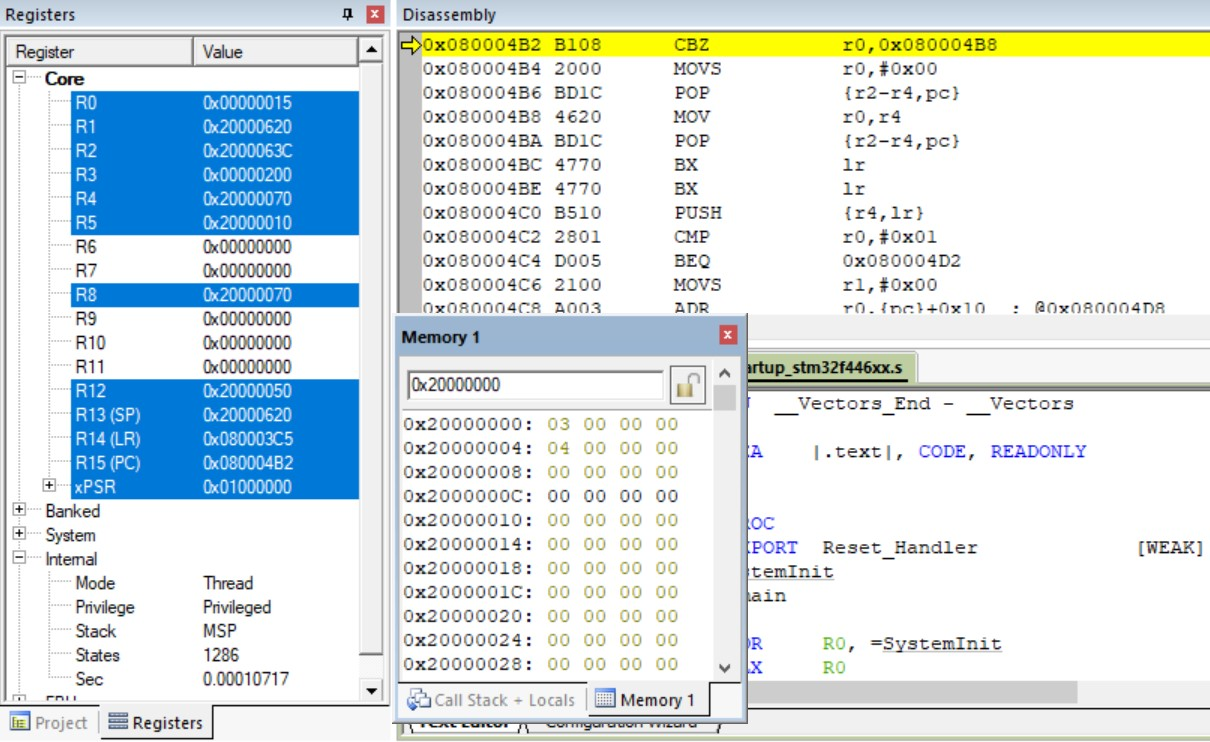
\includegraphics[scale=.7]{images/Task3b_Before1.jpg}
    \caption{After loading the code on the system}
    \label{fig:before_task_3b}
\end{figure}
\FloatBarrier
Here we can see that the registers are loaded with random values as the program is only loaded to the system and not executed yet. But the memory holds the values 0x03 and 0x04 for b and c respectively.
\subsection*{Screenshot of the state of the system after the code has been executed}
\addcontentsline{toc}{subsection}{Screenshot of the state \& status registers of the system after the code has been executed}
\begin{figure}[h!]
    \centering
    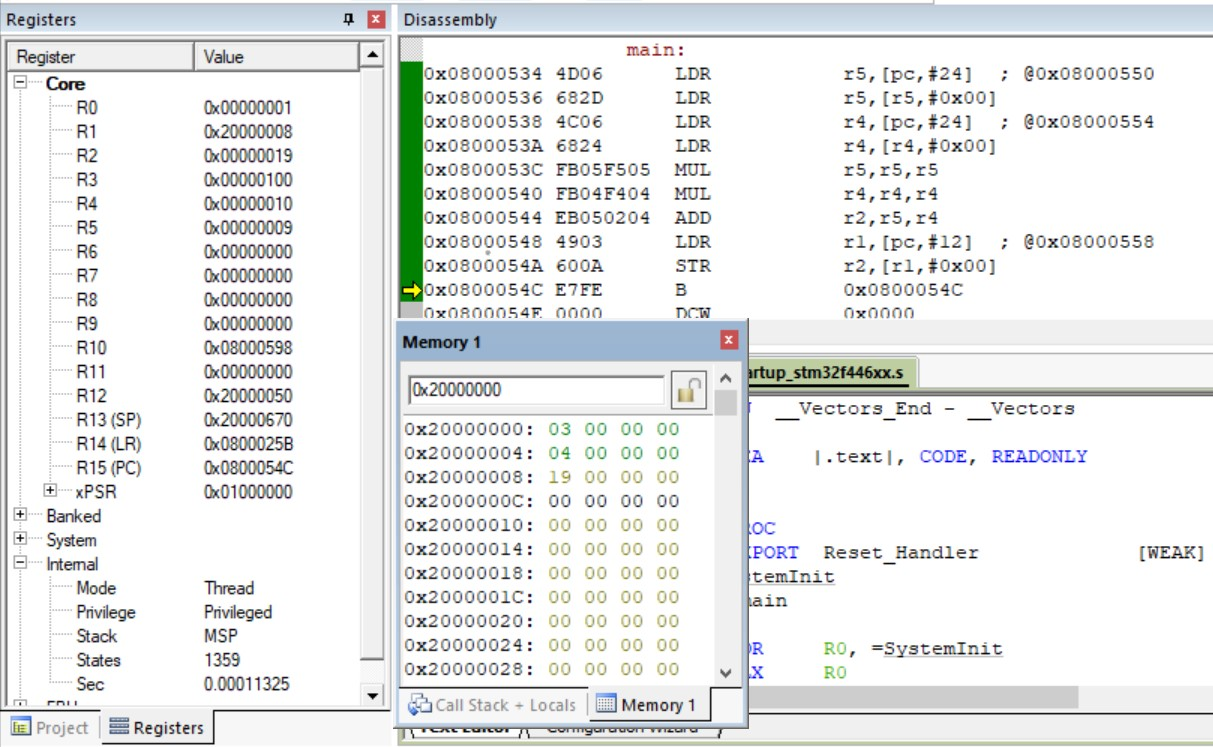
\includegraphics[scale=.7]{images/Task3b_After1.jpg}
    \caption{After executing the code on the system}
    \label{fig:after_task_3b}
\end{figure}
\FloatBarrier
As we can see, the register \$r2 as well as the memory holds the value 0x19, which should be the result of the operation as 25 is equals to hex value 0x19.





%------------------------------------------------------------------------------------
\FloatBarrier
\section*{Task iv(a)}
\addcontentsline{toc}{section}{Task iv(a)}
\addcontentsline{toc}{subsection}{Problem Statement}
\textbf{Problem Statement:} Write assembly program to perform the String operations: Print a String.
\subsection*{Explanation of Code}
\addcontentsline{toc}{subsection}{Explanation of Code}
A string is defined in memory using the DCB instruction, with predefined value "HELL" in this case. The string is loaded into a register to show its contents.
\subsection*{Description of Instructions}
\addcontentsline{toc}{subsection}{Description of Instructions}
\textbf{LDR}\\
The \verb|LDR| pseudo-instruction loads a register with either a 32-bit constant value or an address.\\
\verb|LDR{type}{cond} Rt, [Rn {, #offset}]| \\
\textbf{DCB}\\
The \verb|DCB| directive allocates one or more bytes of memory, and defines the initial runtime contents of the memory.\\
\verb|{label} DCB expr{,expr}...|\\




\FloatBarrier
\subsection*{Screenshot of the state \& status registers of the system after the code has been loaded}
\addcontentsline{toc}{subsection}{Screenshot of the state \& status registers of the system after the code has been loaded}
\begin{figure}[ht]
    \centering
    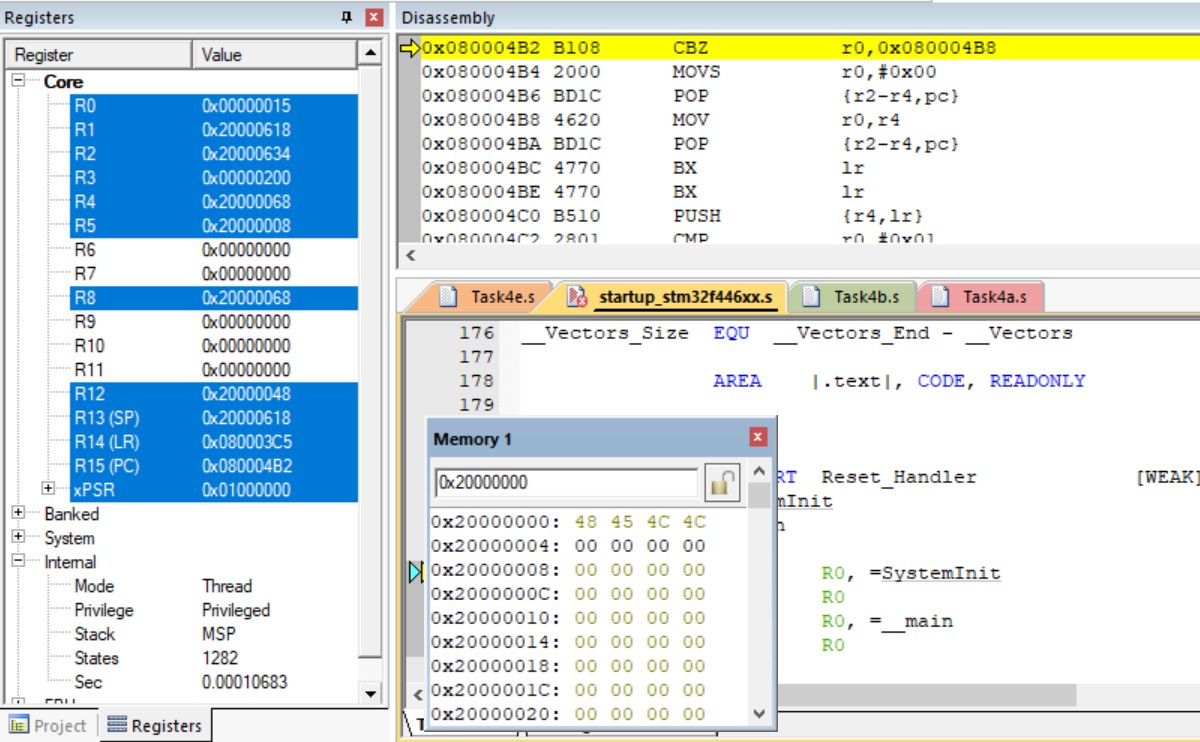
\includegraphics[scale=.7]{images/Task4a_Before1.jpg}
    \caption{After loading the code on the system}
    \label{fig:before_task_4a}
\end{figure}
\FloatBarrier
Here we can see that the registers are loaded with random values as the program is only loaded to the system and not executed yet. But the memory holds the values 0x48, 0x45, 0x4c, 0x4c, which is the binary representation of the string "HELL" in little-endian format.
\subsection*{Screenshot of the state of the system after the code has been executed}
\addcontentsline{toc}{subsection}{Screenshot of the state \& status registers of the system after the code has been executed}
\begin{figure}[h!]
    \centering
    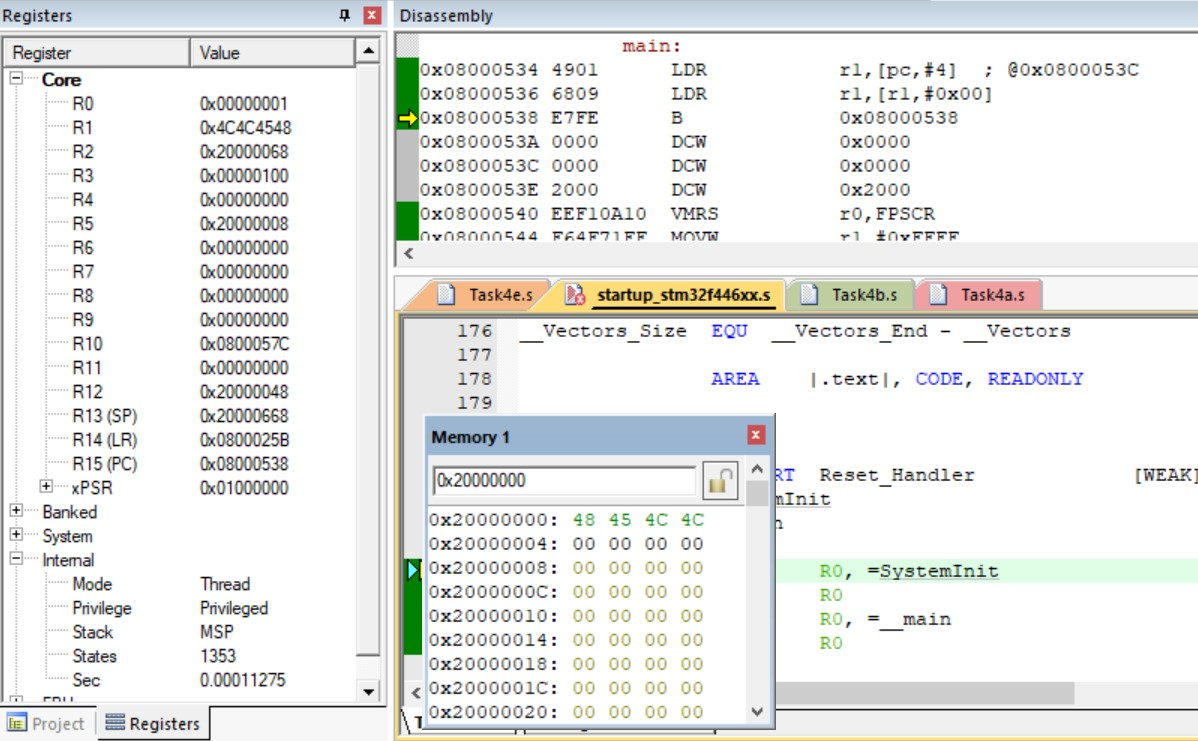
\includegraphics[scale=.7]{images/Task4a_After1.jpg}
    \caption{After executing the code on the system}
    \label{fig:after_task_4a}
\end{figure}
\FloatBarrier
As we can see, the register \$r1 is loaded with the value or the representation of the string that was in the memory.






%------------------------------------------------------------------------------------
\FloatBarrier
\addcontentsline{toc}{section}{Task iv(b)}
\section*{Task iv(b)}
\addcontentsline{toc}{subsection}{Problem Statement}
\textbf{Problem Statement:} Write assembly program to perform the String operations: Reverse a String.
\subsection*{Explanation of Code}
\addcontentsline{toc}{subsection}{Explanation of Code}
Initially, a 0-terminated string is declared with predefined values in memory. The length of the string is calculated, iterating over the characters in the string until a 0-character is reached. Then, we iterate from the left and right point of the string and progress towards the midpoint from both directions, until the pointing indexes bypass each other. During each iteration, the characters in the pointing indexes are swapped, which ultimately results in the reversal of the string.
\subsection*{Description of Instructions}
\addcontentsline{toc}{subsection}{Description of Instructions}
\textbf{LDR}\\
The \verb|LDR| pseudo-instruction loads a register with either a 32-bit constant value or an address.\\
\verb|LDR{type}{cond} Rt, [Rn {, #offset}]| \\
\textbf{MOV}\\
The \verb|MOV| instruction copies the value of \verb|Operand2| into \verb|Rd|.\\
\verb|MOV{S}{cond} Rd, Operand2|\\
\verb|MOV{cond} Rd, #imm16|\\
\textbf{ADD}\\
The \verb|ADD| instruction adds the values in Rn and Operand2 or imm12. \verb|S| is an optional suffix. If \verb|S| is specified, the condition flags are updated on the result of the operation.\\
\verb|ADD{S}{cond} {Rd}, Rn, Operand2|\\
\textbf{SUB}\\
The \verb|SUB| instruction subtracts the value of Operand2 or imm12 from the value in Rn. If \verb|S| is specified, the condition flags are updated on the result of the operation.\\
\verb|SUB{S}{cond} {Rd}, Rn, Operand2|\\
\textbf{LDRB}\\
The \verb|LDRB| instruction calculates an address from a base register value and an offset register value, loads a byte from memory, zero-extends it to form a 32-bit word, and writes it to a register. \\
\verb|LDRB<c> <Rt>, [<Rn>, <Rm>]|\\
\textbf{STRB}\\
The \verb|STRB| instruction calculates an address from a base register value and an offset register value, and stores a byte from a register to memory. \\
\verb|STRB<c> <Rt>, [<Rn>, <Rm>]|\\
\textbf{B}\\
The \verb|B| instruction performs a branch to a label.\\
\verb|B{cond}{.W} label|\\
\textbf{BEQ}\\
The \verb|BEQ| instruction performs a conditional branch to a label if the flag set by an equality check is true.\\
\verb|BEQ {.W} label|\\
\textbf{CMP}\\
The \verb|CMP| instruction subtracts the value of Operand2 from the value in Rn. This is the same as a \verb|SUBS| instruction, except that the result is discarded.\\
\verb|CMP{cond} Rn, Operand2|\\
\textbf{BHS}\\
The \verb|BHS| instruction performs a conditional branch to a label if the flag set by a check, if an unsigned value is greater or same, is true.\\
\verb|BHS {.W} label|\\
\textbf{DCDU}\\
The \verb|DCD| directive allocates one or more words of memory, aligned on four-byte boundaries, and defines the initial runtime contents of the memory.\verb|DCDU| is the same, except that the memory alignment is arbitrary.\\
\verb|{label} DCDU expr{,expr}|\\


\FloatBarrier
\subsection*{Screenshot of the state \& status registers of the system after the code has been loaded}
\addcontentsline{toc}{subsection}{Screenshot of the state \& status registers of the system after the code has been loaded}
\begin{figure}[ht]
    \centering
    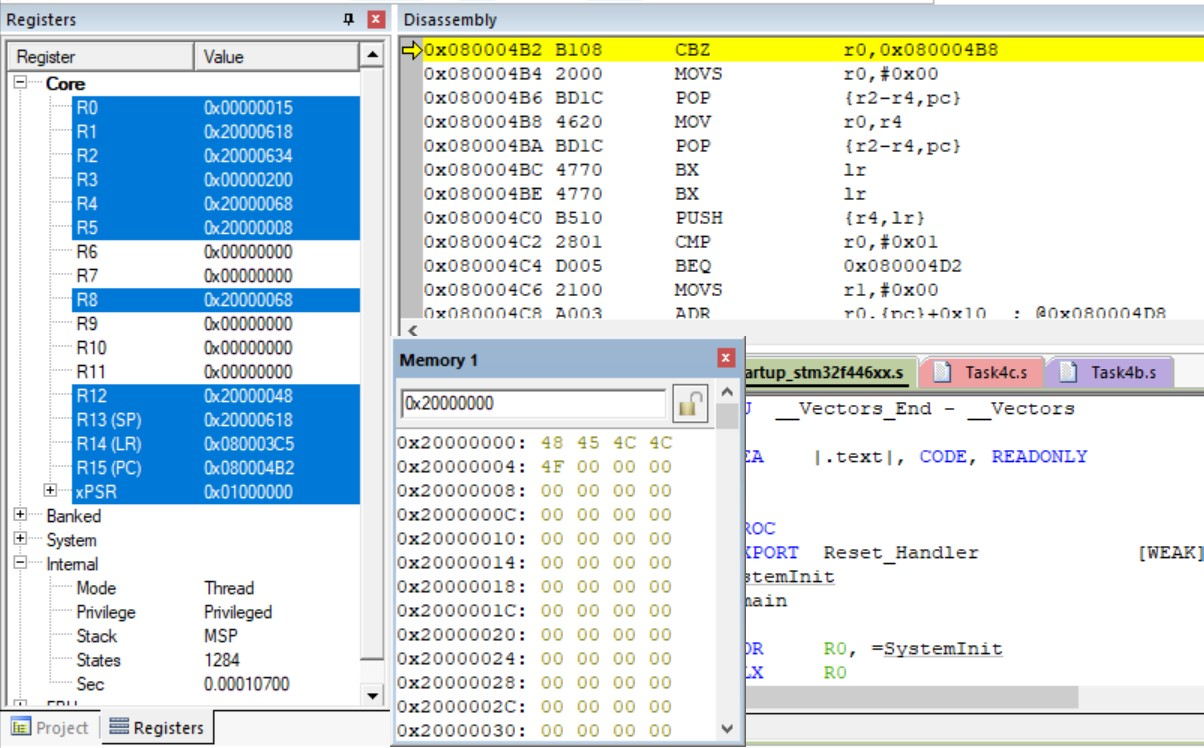
\includegraphics[scale=.7]{images/Task4b_Before1.jpg}
    \caption{After loading the code on the system}
    \label{fig:before_task_4b}
\end{figure}
\FloatBarrier
Here we can see that the registers are loaded with random values as the program is only loaded to the system and not executed yet. But the memory holds the values 0x48, 0x45, 0x4c, 0x4c and 0x4f, which is the binary representation of the string "HELLO" in little-endian format.
\subsection*{Screenshot of the state of the system after the code has been executed}
\addcontentsline{toc}{subsection}{Screenshot of the state \& status registers of the system after the code has been executed}
\begin{figure}[h!]
    \centering
    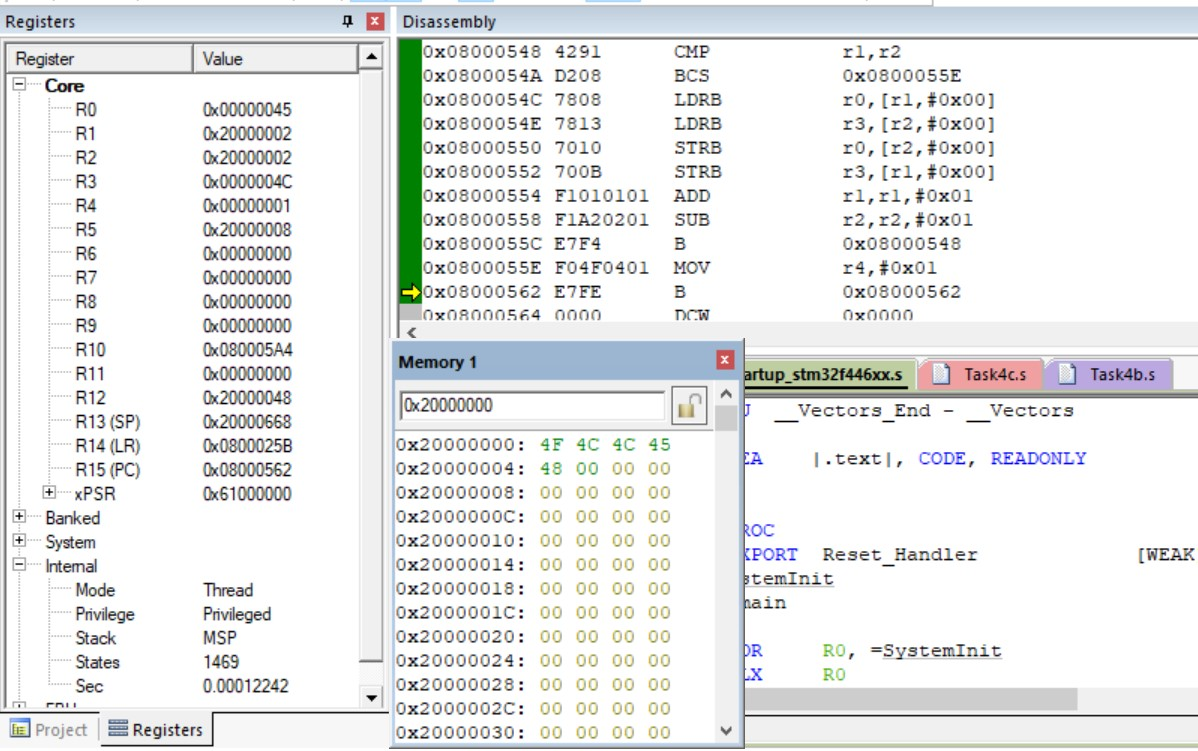
\includegraphics[scale=.7]{images/Task4b_After1.jpg}
    \caption{After executing the code on the system}
    \label{fig:after_task_4b}
\end{figure}
\FloatBarrier
As we can see, the memory has the previous string representation reversed after the execution of the code.


%------------------------------------------------------------------------------------
%------------------------------------------------------------------------------------
\FloatBarrier
\addcontentsline{toc}{section}{Task iv(c)}
\section*{Task iv(c)}
\addcontentsline{toc}{subsection}{Problem Statement}
\textbf{Problem Statement:} Write assembly program to perform the String operations: Length of a String.
\subsection*{Explanation of Code}
\addcontentsline{toc}{subsection}{Explanation of Code}
A 0-terminated string (with a predefined value) and a variable (for storing the length of the string) is declared initially. After loading the string into a register, we start iterating from the first character until we find the terminating 0-character, increasing the result for the length in each iteration by 1. Finally, the result is stored into memory.
\subsection*{Description of Instructions}
\addcontentsline{toc}{subsection}{Description of Instructions}
\textbf{LDR}\\
The \verb|LDR| pseudo-instruction loads a register with either a 32-bit constant value or an address.\\
\verb|LDR{type}{cond} Rt, [Rn {, #offset}]| \\
\textbf{STR}\\
The \verb|STR| pseudo-instruction loads a register with values from either a 32-bit constant or an address.\\
\verb|STR{type}{cond} Rt, [Rn {, #offset}]|\\  
\textbf{ADD}\\
The \verb|ADD| instruction adds the values in Rn and Operand2 or imm12. \verb|S| is an optional suffix. If \verb|S| is specified, the condition flags are updated on the result of the operation.\\
\verb|ADD{S}{cond} {Rd}, Rn, Operand2|\\
\textbf{B}\\
The \verb|B| instruction performs a branch to a label.\\
\verb|B{cond}{.W} label|\\
\textbf{BEQ}\\
The \verb|BEQ| instruction performs a conditional branch to a label if the flag set by an equality check is true.\\
\verb|BEQ {.W} label|\\
\textbf{CMP}\\
The \verb|CMP| instruction subtracts the value of Operand2 from the value in Rn. This is the same as a \verb|SUBS| instruction, except that the result is discarded.\\
\verb|CMP{cond} Rn, Operand2|\\
\textbf{DCDU}\\
The \verb|DCD| directive allocates one or more words of memory, aligned on four-byte boundaries, and defines the initial runtime contents of the memory.\verb|DCDU| is the same, except that the memory alignment is arbitrary.\\
\verb|{label} DCDU expr{,expr}|\\


\FloatBarrier
\subsection*{Screenshot of the state \& status registers of the system after the code has been loaded}
\addcontentsline{toc}{subsection}{Screenshot of the state \& status registers of the system after the code has been loaded}
\begin{figure}[ht]
    \centering
    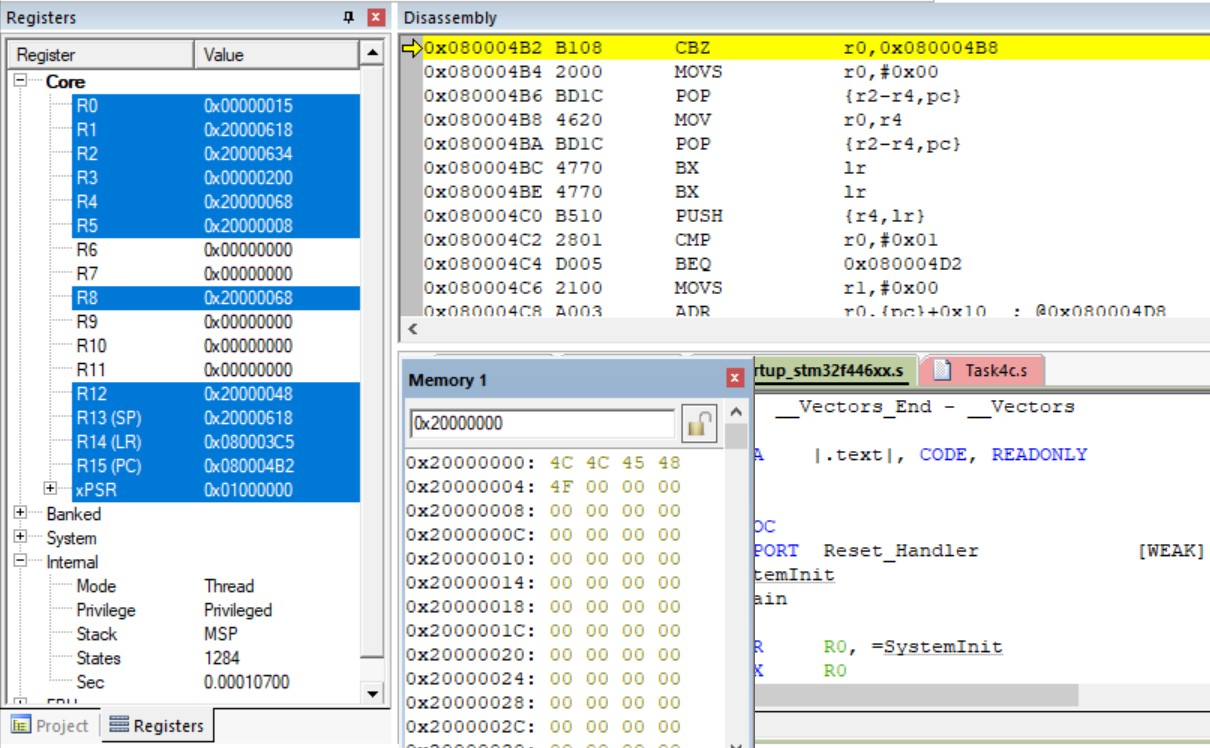
\includegraphics[scale=.7]{images/Task4c_Before1.jpg}
    \caption{After loading the code on the system}
    \label{fig:before_task_4c}
\end{figure}
\FloatBarrier
Here we can see that the registers are loaded with random values as the program is only loaded to the system and not executed yet. But the memory holds the values 0x48, 0x45, 0x4c, 0x4c and 0x4f, which is the binary representation of the string "HELLO" in little-endian format.
\subsection*{Screenshot of the state of the system after the code has been executed}
\addcontentsline{toc}{subsection}{Screenshot of the state \& status registers of the system after the code has been executed}
\begin{figure}[h!]
    \centering
    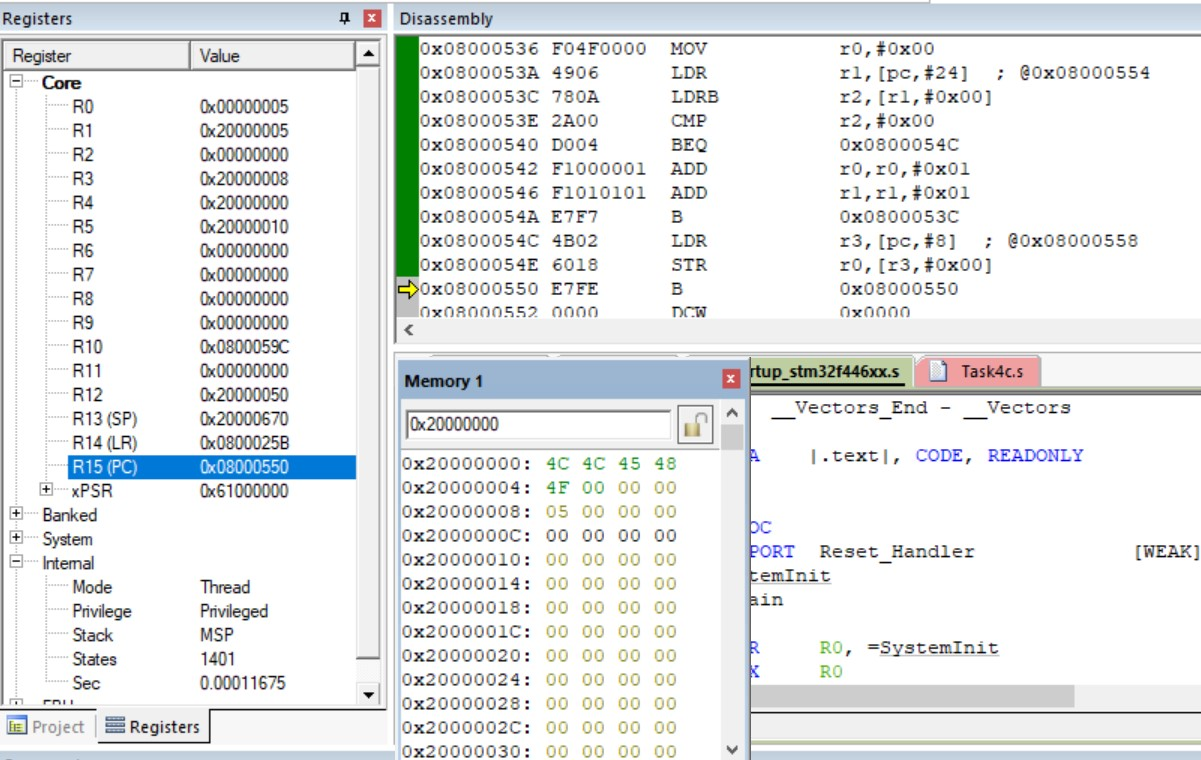
\includegraphics[scale=.7]{images/Task4c_After1.jpg}
    \caption{After executing the code on the system}
    \label{fig:after_task_4c}
\end{figure}
\FloatBarrier
As we can see, the register \$r0 and memory(0x20000008) has length of the string, which is 5 in this case, stored after the execution of the code.






%----------------------------------------------------------------------------------------
\FloatBarrier
\addcontentsline{toc}{section}{Task iv(d)}
\section*{Task iv(d)}
\addcontentsline{toc}{subsection}{Problem Statement}
\textbf{Problem Statement:} Write assembly program to perform the String operations: Compare two String and show the status of PSR.
\subsection*{Explanation of Code}
\addcontentsline{toc}{subsection}{Explanation of Code}
Two strings with predefined values are defined in memory. After loading them into two registers, we start comparing them character by character, until both of them are empty simultaneously. If a position is found, where one character in a string differs from the character in the same index of the other string, we update flags for greater than or less than conditions and exit the loop.
\subsection*{Description of Instructions}
\addcontentsline{toc}{subsection}{Description of Instructions}
\textbf{LDR}\\
The \verb|LDR| pseudo-instruction loads a register with either a 32-bit constant value or an address.\\
\verb|LDR{type}{cond} Rt, [Rn {, #offset}]| \\
\textbf{LDRB}\\
The \verb|LDRB| instruction calculates an address from a base register value and an offset register value, loads a byte from memory, zero-extends it to form a 32-bit word, and writes it to a register. \\
\verb|LDRB<c> <Rt>, [<Rn>, <Rm>]|\\\textbf{ADD}\\
The \verb|ADD| instruction adds the values in Rn and Operand2 or imm12. \verb|S| is an optional suffix. If \verb|S| is specified, the condition flags are updated on the result of the operation.\\
\verb|ADD{S}{cond} {Rd}, Rn, Operand2|\\
\textbf{ORR}\\
The \verb|ORR| instruction performs bitwise \verb|ORR| operations on the values in Rn and Operand2.\\
\verb|ORR{S}{cond} Rd, Rn, Operand2|\\
\textbf{MOVGT}
The \verb|MOVGT| instruction performs a conditional move, in case of the flag modified by a check for greater than (signed comparison) is set accordingly.
\verb|MOVGT Rd, #imm|
\textbf{MOVLT}
The \verb|MOVLT| instruction performs a conditional move, in case of the flag modified by a check for less than (signed comparison) is set accordingly.
\verb|MOVLT Rd, #imm|
\textbf{BEQ}\\
The \verb|BEQ| instruction performs a conditional branch to a label if the flag set by an equality check is true.\\
\verb|BEQ {.W} label|\\
\textbf{CMP}\\
The \verb|CMP| instruction subtracts the value of Operand2 from the value in Rn. This is the same as a \verb|SUBS| instruction, except that the result is discarded.\\
\verb|CMP{cond} Rn, Operand2|\\
\textbf{DCB}\\
The \verb|DCB| directive allocates one or more bytes of memory, and defines the initial runtime contents of the memory.\\
\verb|{label} DCB expr{,expr}...|\\










\FloatBarrier
\subsection*{Screenshot of the state \& status registers of the system after the code has been loaded}
\addcontentsline{toc}{subsection}{Screenshot of the state \& status registers of the system after the code has been loaded}
\begin{figure}[ht]
    \centering
    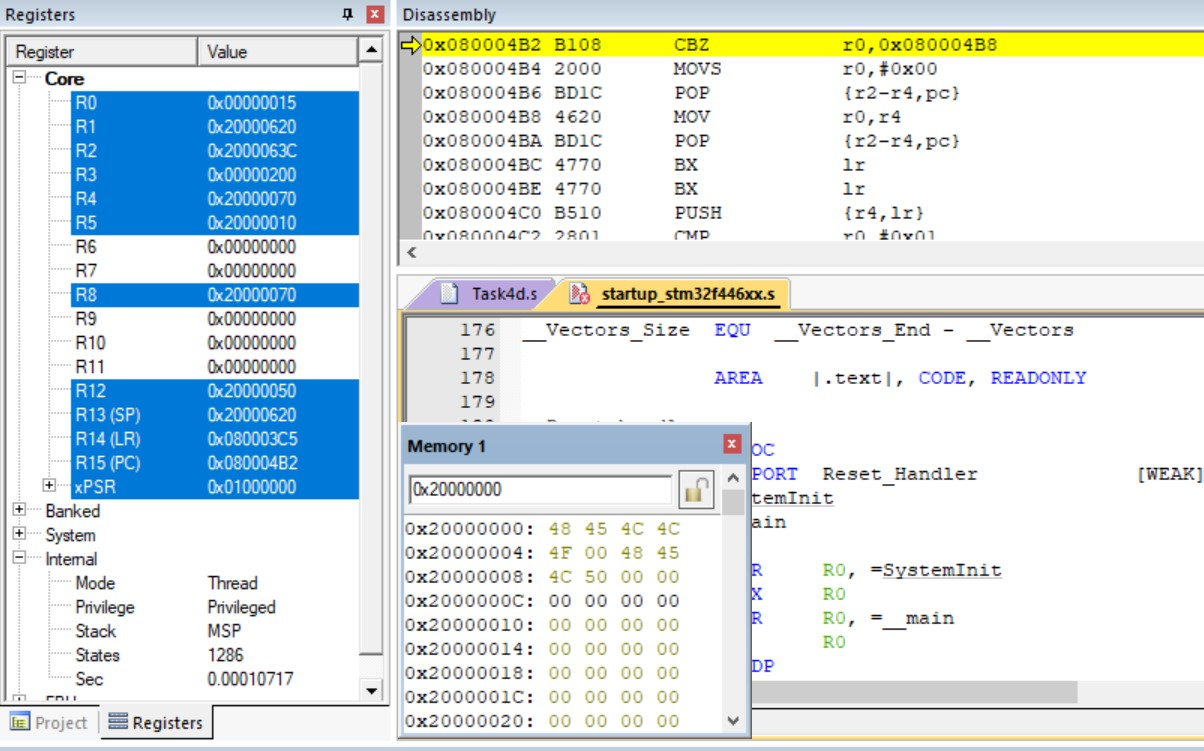
\includegraphics[scale=.7]{images/Task4d_Before1.jpg}
    \caption{After loading the code on the system}
    \label{fig:before_task_4d}
\end{figure}
\FloatBarrier
Here we can see that the registers are loaded with random values as the program is only loaded to the system and not executed yet. But the memory holds the values 0x48, 0x45, 0x4c, 0x4c and 0x4f, which is the binary representation of the string "HELLO" in little-endian format and after a terminating 0, the values 0x48, 0x45, 0x4c, 0x50, which is the binary representation of the string "HELP" in little-endian format.
\subsection*{Screenshot of the state of the system after the code has been executed}
\addcontentsline{toc}{subsection}{Screenshot of the state \& status registers of the system after the code has been executed}
\begin{figure}[h!]
    \centering
    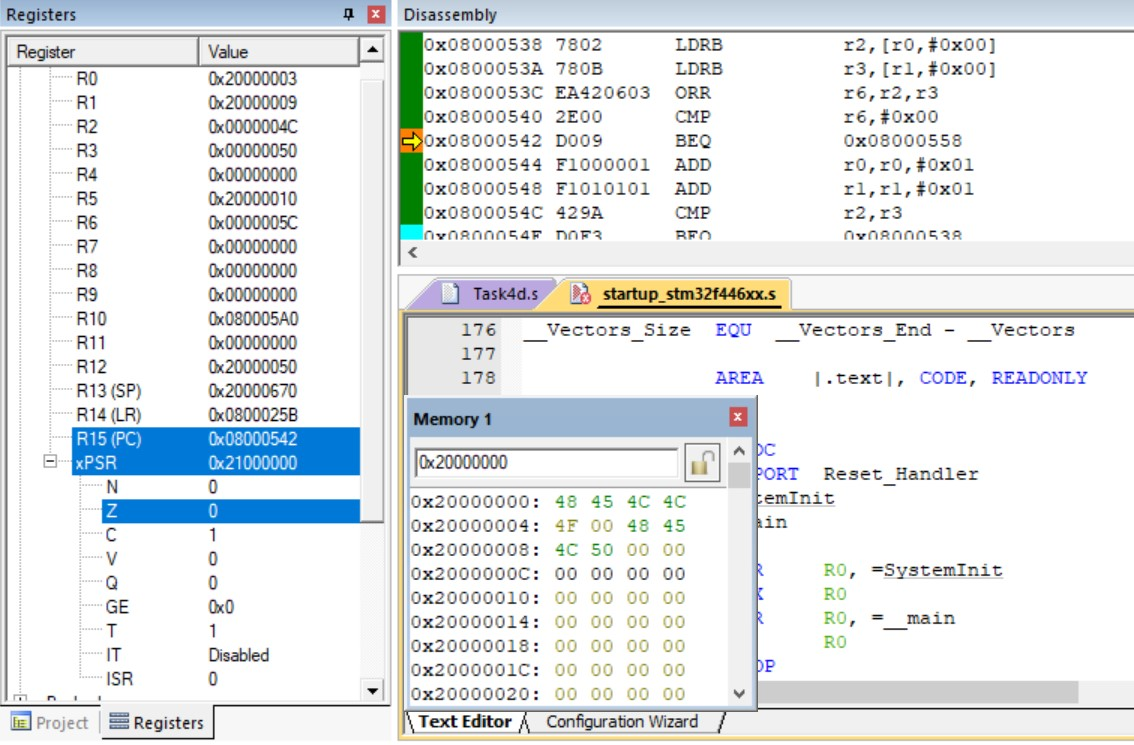
\includegraphics[scale=.7]{images/Task4d_After1.jpg}
    \caption{After executing the code on the system}
    \label{fig:after_task_4d1}
\end{figure}
\FloatBarrier
As we can see, as a result of comparison between characters 'L' and 'P', the PSR registers have changed value which indicated 'P'>'L' (Conditional suffix: LT). Which means we can now branch to the decision logic for str(a) < str(b).
\addcontentsline{toc}{subsection}{Screenshot of the state \& status registers of the system after the code has been executed}
\begin{figure}[h!]
    \centering
    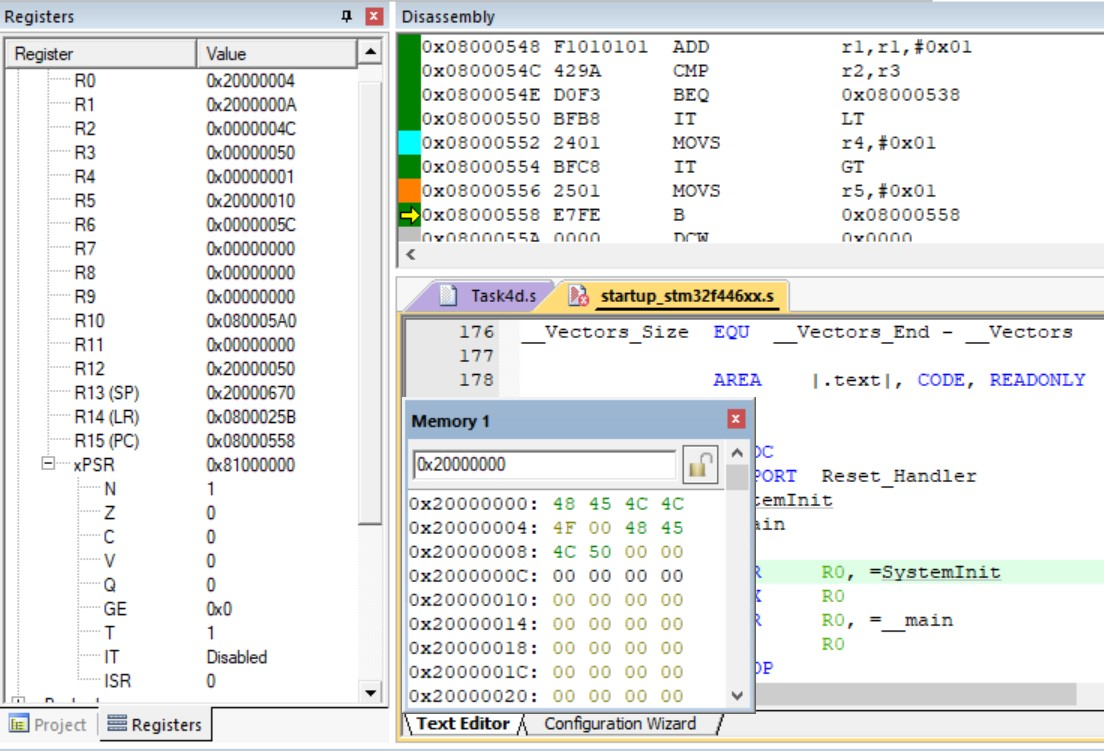
\includegraphics[scale=.7]{images/Task4d_After2.jpg}
    \caption{After executing the code on the system}
    \label{fig:after_task_4d2}
\end{figure}
\FloatBarrier
As we can see, as a result of comparison between strings 'HELLO' and 'HELP', we have set the register \$r4 to 1, as we branced to that logic using the xPSR registers values (as shown in the previous screenshot).













%------------------------------------------------------------------------------------------
\FloatBarrier
\addcontentsline{toc}{section}{Task iv(e)}
\section*{Task iv(e)}
\addcontentsline{toc}{subsection}{Problem Statement}
\textbf{Problem Statement:} Write assembly program to perform the String operations: Concatenate two Strings.
\subsection*{Explanation of Code}
\addcontentsline{toc}{subsection}{Explanation of Code}
Two 0-terminated strings with predefined values and an empty string are declared in memory. After loading the first string in a register, we keep iterating from the first character until we find the terminating 0-character, adding the current character to the previously declared empty string. After this loop ends, we follow the same process for the second string, starting by loading it in a register and finishing after adding all characters to the string which was initialized as empty. Finally, the resultant string is stored in memory.
\subsection*{Description of Instructions}
\addcontentsline{toc}{subsection}{Description of Instructions}
\textbf{LDR}\\
The \verb|LDR| pseudo-instruction loads a register with either a 32-bit constant value or an address.\\
\verb|LDR{type}{cond} Rt, [Rn {, #offset}]| \\
\textbf{LDRB}\\
The \verb|LDRB| instruction calculates an address from a base register value and an offset register value, loads a byte from memory, zero-extends it to form a 32-bit word, and writes it to a register. \\
\verb|LDRB<c> <Rt>, [<Rn>, <Rm>]|\\
\textbf{STRB}\\
The \verb|STRB| instruction calculates an address from a base register value and an offset register value, and stores a byte from a register to memory. \\
\verb|STRB<c> <Rt>, [<Rn>, <Rm>]|\\
\textbf{MOV}\\The \verb|MOV| instruction copies the value of \verb|Operand2| into \verb|Rd|.\\
\verb|MOV{S}{cond} Rd, Operand2|\\
\verb|MOV{cond} Rd, #imm16|\\
\textbf{ADD}\\
The \verb|ADD| instruction adds the values in Rn and Operand2 or imm12. \verb|S| is an optional suffix. If \verb|S| is specified, the condition flags are updated on the result of the operation.\\
\verb|ADD{S}{cond} {Rd}, Rn, Operand2|\\
\textbf{B}\\
The \verb|B| instruction performs a branch to a label.\\
\verb|B{cond}{.W} label|\\
\textbf{BEQ}\\
The \verb|BEQ| instruction performs a conditional branch to a label if the flag set by an equality check is true.\\
\verb|BEQ {.W} label|\\
\textbf{CMP}\\
The \verb|CMP| instruction subtracts the value of Operand2 from the value in Rn. This is the same as a \verb|SUBS| instruction, except that the result is discarded.\\
\verb|CMP{cond} Rn, Operand2|\\
\textbf{DCB}\\
The \verb|DCB| directive allocates one or more bytes of memory, and defines the initial runtime contents of the memory.\\
\verb|{label} DCB expr{,expr}...|\\



\FloatBarrier
\subsection*{Screenshot of the state \& status registers of the system after the code has been loaded}
\addcontentsline{toc}{subsection}{Screenshot of the state \& status registers of the system after the code has been loaded}
\begin{figure}[ht]
    \centering
    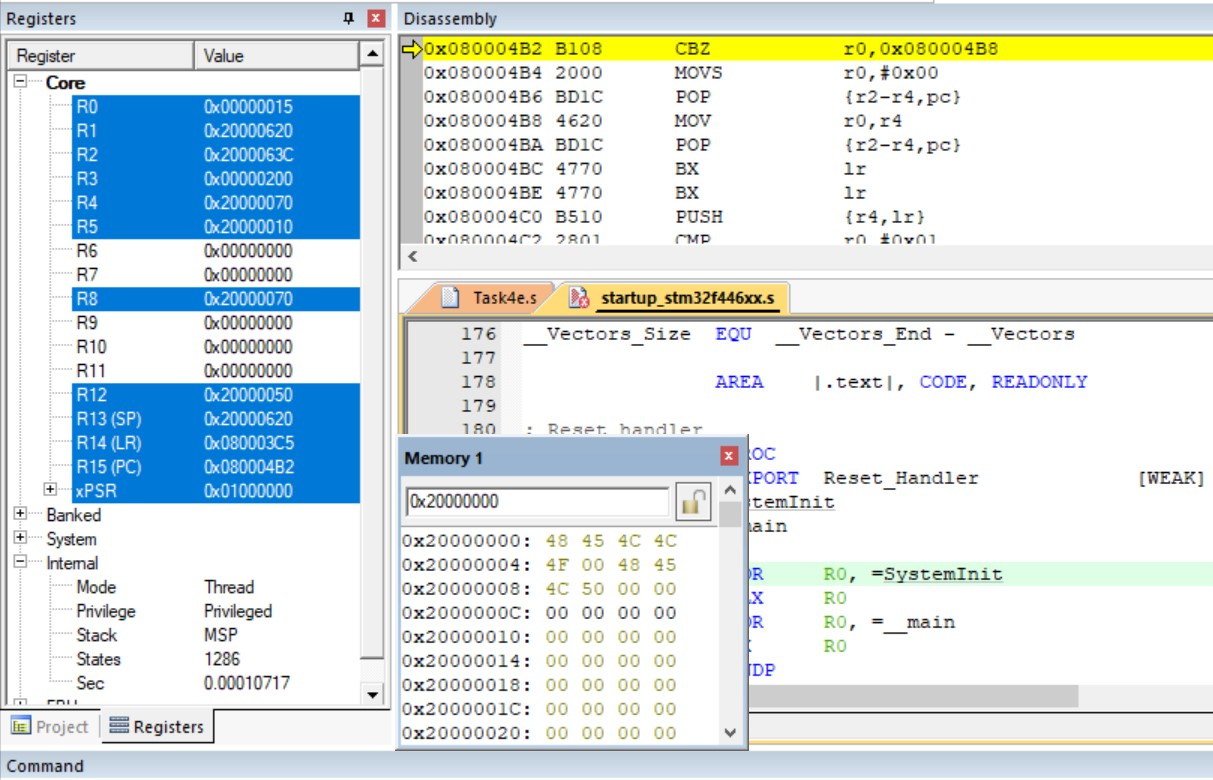
\includegraphics[scale=.7]{images/Task4e_Before1.jpg}
    \caption{After loading the code on the system}
    \label{fig:before_task_4e}
\end{figure}
\FloatBarrier
Here we can see that the registers are loaded with random values as the program is only loaded to the system and not executed yet. But the memory holds the values 0x48, 0x45, 0x4c, 0x4c and 0x4f, which is the binary representation of the string "HELLO" in little-endian format and after a terminating 0, the values 0x48, 0x45, 0x4c, 0x50, which is the binary representation of the string "HELP" in little-endian format.
\subsection*{Screenshot of the state of the system after the code has been executed}
\addcontentsline{toc}{subsection}{Screenshot of the state \& status registers of the system after the code has been executed}
\begin{figure}[h!]
    \centering
    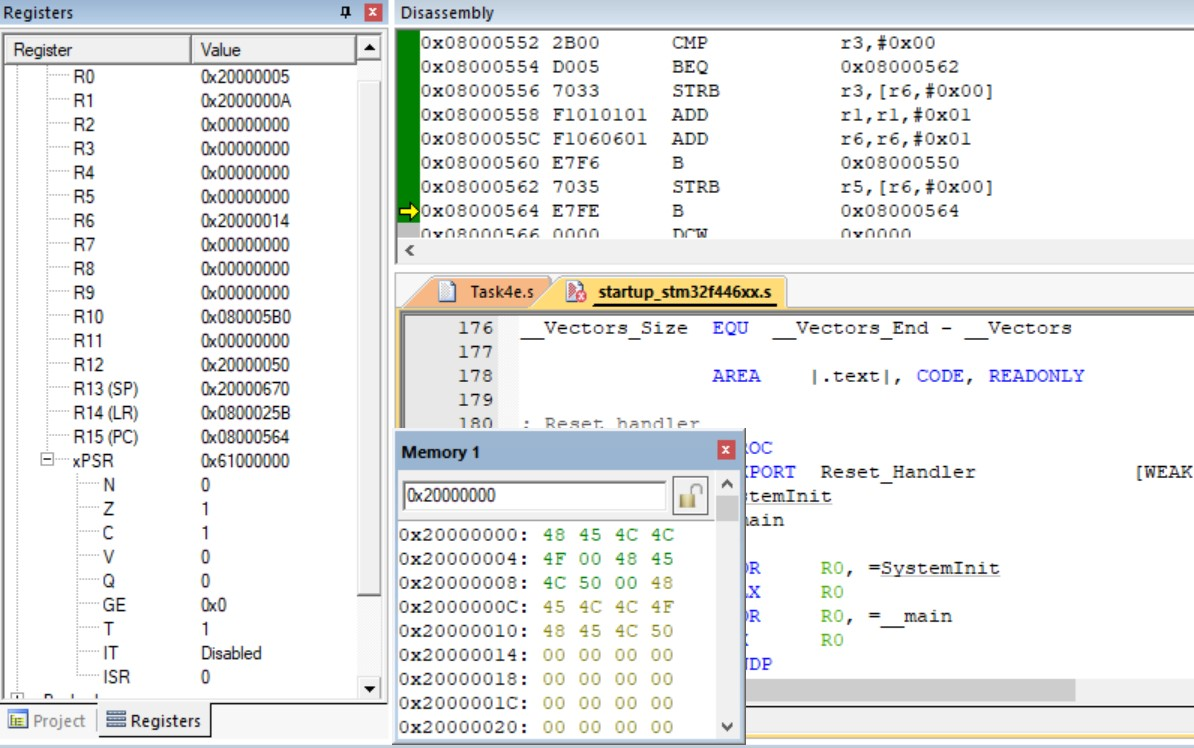
\includegraphics[scale=.7]{images/Task4e_After1.jpg}
    \caption{After executing the code on the system}
    \label{fig:after_task_4e}
\end{figure}
\FloatBarrier
As we can see, the memory(0x20000008) has the concatenated string as values 0x48, 0x45, 0x4c, 0x4c, 0x4f, 0x48, 0x45, 0x4c, 0x50, which is the hex representation of "HELLOHELP", and it ends with a terminating 0.


%------------------------------------------------------------------------------------------
\end{document}